\documentclass{article}
\usepackage[utf8]{inputenc}
\usepackage{amsmath,amssymb}
\usepackage{graphicx}
\usepackage{float}
\usepackage{subcaption}
\usepackage{geometry}
\geometry{
    a4paper,
    total={170mm,257mm},
    left=20mm,
    right=20mm,
    top=20mm,
}
\usepackage{listings} % code listings
\lstset{framextopmargin=0pt,frame=lines}
\lstset{
    language=Matlab,
    basicstyle=\footnotesize\ttfamily,
    breaklines=true,
    tabsize=4,
    keepspaces=true,
    columns=flexible,
    % backgroundcolor=\color[gray]{0.9},
    frame=single,
    breaklines=true,%
    morekeywords={matlab2tikz},
    keywordstyle=\color{blue},%
    morekeywords=[2]{1}, keywordstyle=[2]{\color{black}},
    identifierstyle=\color{black},%
    stringstyle=\color{mylilas},
    commentstyle=\color{mygreen},%
    showstringspaces=false,%without this there will be a symbol in the places where there is a space
    numbers=left,
    numberstyle={\tiny \color{black}},% size of the numbers
    numbersep=9pt, % this defines how far the numbers are from the text
    emph=[1]{for,end,break},emphstyle=[1]\color{red}, %some words to emphasise
    %emph=[2]{word1,word2}, emphstyle=[2]{style},
}
\usepackage{color} %red, green, blue, yellow, cyan, magenta, black, white
\definecolor{mygreen}{RGB}{28,172,0} % color values Red, Green, Blue
\definecolor{mylilas}{RGB}{170,55,241}

\title{ENV-541 Sensor Orientation\\Lab 4 - Inertial Navigation in 2D / Nominal Signal}
\author{Michael Spieler}
\date{October 26, 2018}

\begin{document}

\maketitle

\section*{Strapdown inertial navigation}

The simulated sensor samples are in the body frame and must be transformed to the inertial map frame.

\begin{equation*}
\omega_{mb}^b = \begin{bmatrix} \omega_0 \end{bmatrix}
\end{equation*}

\begin{equation*}
f^m = R_b^m(\alpha) f^b = \begin{bmatrix} 0 \\ r \omega_0^2 \end{bmatrix}
\end{equation*}

\begin{equation*}
R_b^m(\alpha) = \begin{bmatrix}
    \cos(\alpha) & -\sin(\alpha) \\
    \sin(\alpha) & \cos(\alpha)
    \end{bmatrix}
\end{equation*}

The problem can be formulated as a differential equation which can be integrated numerically:

\begin{align*}
\dot \alpha = \omega_0 \\
\dot v^m = f^m \\
\dot x^m = v^m
\end{align*}

\subsection*{1st order rectangular integration}

\begin{equation*}
x_k = x_{k-1} + \dot x_k \Delta t 
\end{equation*}

\subsection*{2nd order trapezoidal integration}

\begin{equation*}
x_k = x_{k-1} + \frac{1}{2}(\dot x_k + \dot x_{k-1}) \Delta t 
\end{equation*}

The errors of the simulated trajectory using the two integration methods at 10Hz and 100Hz are shown
in figure \ref{fig:error_10hz} and figure \ref{fig:error_100hz}.

\section*{Error plots}
\begin{figure}[H]
    \centering
    \begin{subfigure}[t]{0.49\textwidth}
        \centering
        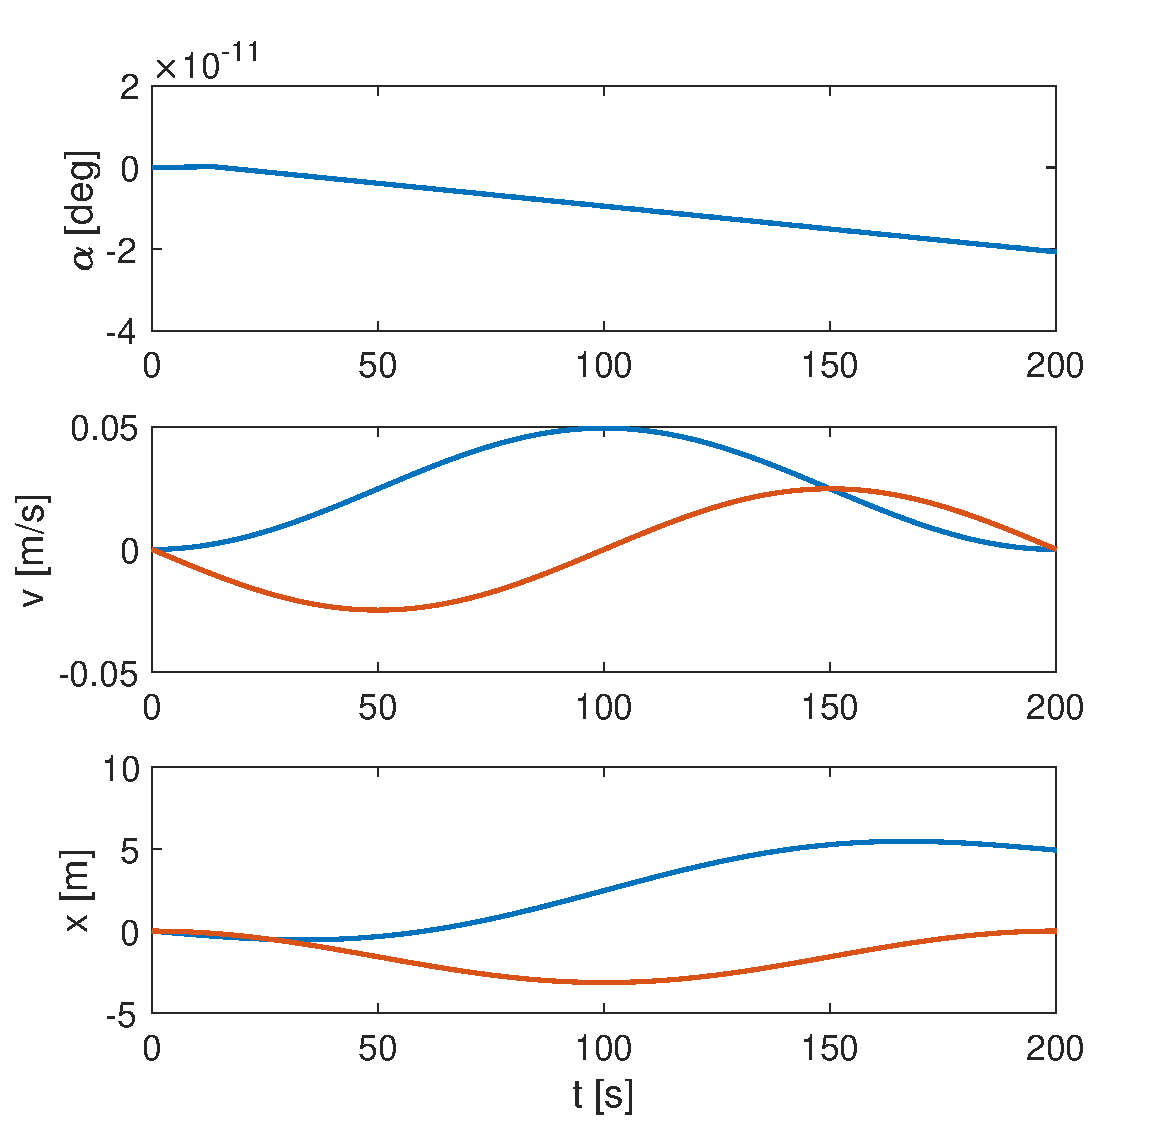
\includegraphics[width=\textwidth]{rectangular_int_10hz}
        \caption{Rectangular integration}
    \end{subfigure}
    ~
    \begin{subfigure}[t]{0.49\textwidth}
        \centering
        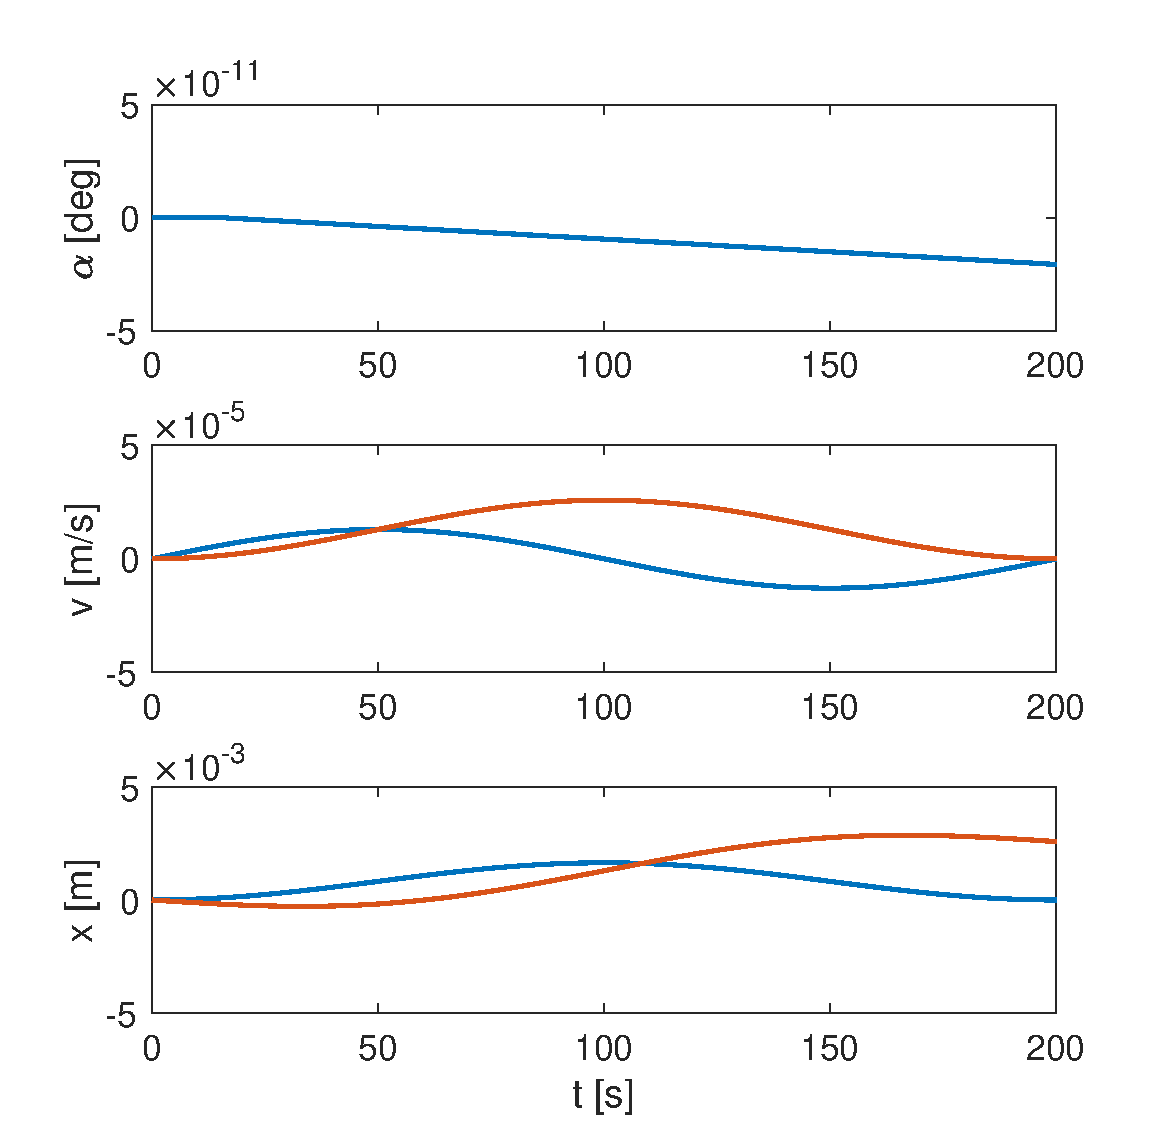
\includegraphics[width=\textwidth]{trapezoidal_int_10hz}
        \caption{Trapezoidal integration}
    \end{subfigure}
    \caption{Trajectory errors at 10Hz sampling rate}
    \label{fig:error_10hz}
\end{figure}

\begin{figure}[H]
    \centering
    \begin{subfigure}[t]{0.49\textwidth}
        \centering
        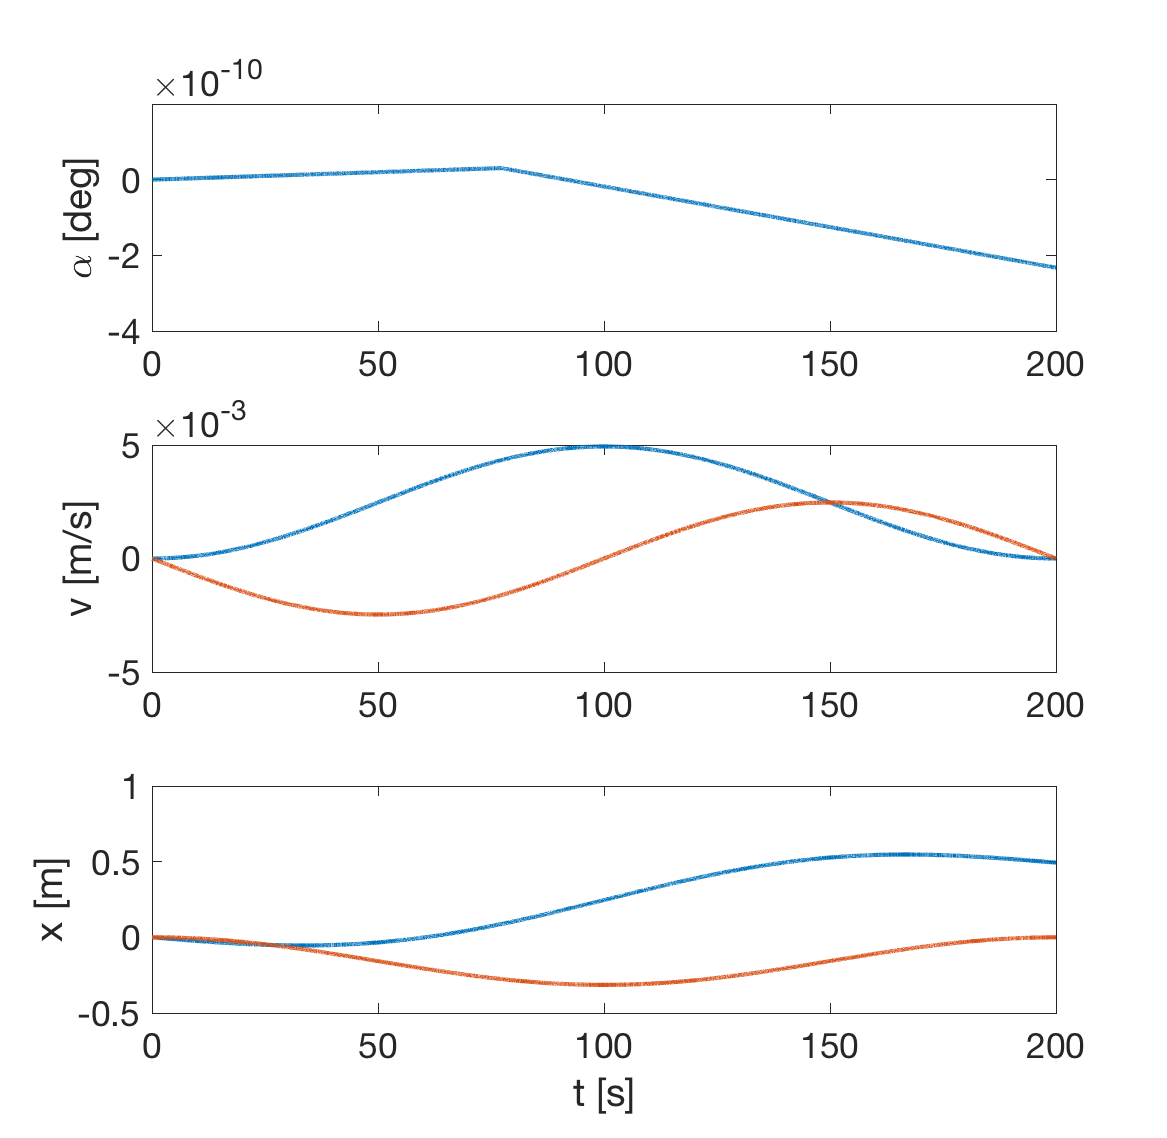
\includegraphics[width=\textwidth]{rectangular_int_100hz}
        \caption{Rectangular integration}
    \end{subfigure}
    ~
    \begin{subfigure}[t]{0.49\textwidth}
        \centering
        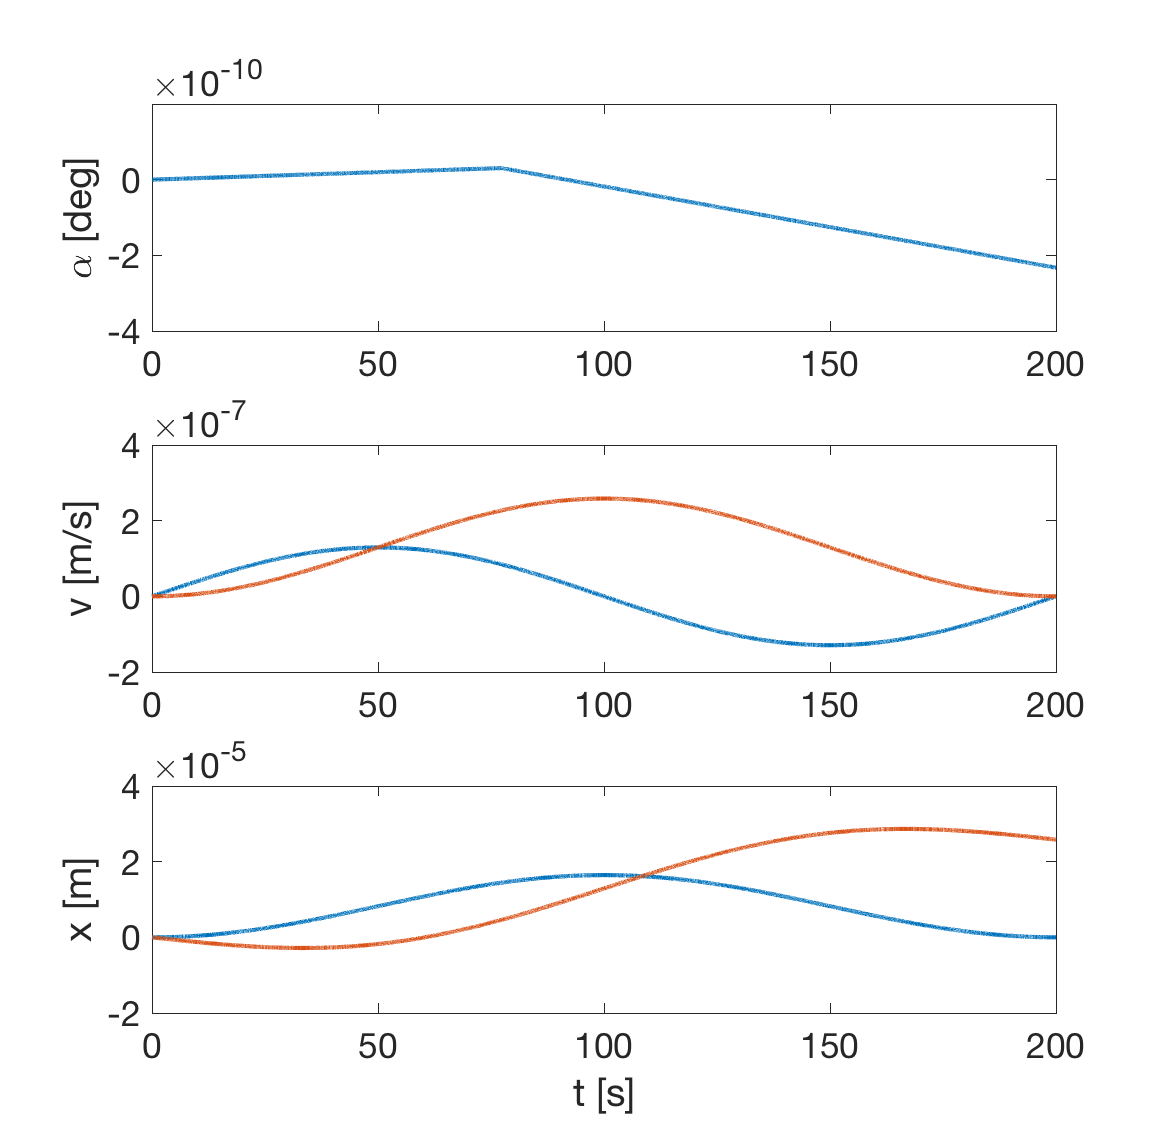
\includegraphics[width=\textwidth]{trapezoidal_int_100hz}
        \caption{Trapezoidal integration}
    \end{subfigure}
    \caption{Trajectory errors at 100Hz sampling rate}
    \label{fig:error_100hz}
\end{figure}

\section*{Trajectory error}

Table \ref{tab:err} shows the maximal trajectory errors in velocity an position for 1st and 2nd order integration at 10Hz and 100Hz sampling frequency.
In general, the higher order integration method and higher sampling rates have the lowest error.

The 1st order rectangular integration is not suited for this application, since it assumes constant derivatives.
Trapezoideal integration gives alredy better results.
However, the nonlinear nature of rotations still results in errors.
Errors can be kept low by using a high sampling rate.

Note: The asimuth error is not listed, since it is zero for all integration methods (the error plots show a small error, which is due to numerical errors during floating point calculations).
This is not surprising, since the angular rate is constant and thus a 1st order integration is perfectly sufficient.

\begin{table}[h]
\centering
\begin{tabular}{lllll}
Error & Rectangular 10Hz & Trapezoidal 10Hz & Rectangular 100Hz & Trapezoidal 100Hz \\
\hline
Velocity x [m/s] & 4.935e-02 & 1.292e-05 & 4.935e-03 & \textbf{1.292e-07} \\
Velocity y [m/s] & 2.469e-02 & 2.584e-05 & 2.468e-03 & \textbf{2.584e-07} \\
Position x [m] & 5.474 & 1.645e-03 & 5.473e-01 & \textbf{1.645e-05} \\
Position y [m] & 3.140 & 2.865e-03 & 3.141e-01 & \textbf{2.865e-05}
\end{tabular}
\caption{Maximal errors during trajectory}
\label{tab:err}
\end{table}

% \newpage
\section*{Code}
\lstinputlisting{../lab4.m}

\end{document}
